\problemname{Bodenschätze}

\illustration{.3}{img/turnbull.jpg}{Eine erodierte Schlammwand legt neue Mineralien frei. Foto: Michael D.\ Turnbull, Lizenz: CC BY-SA.}

\noindent
Du bist für die Signalverarbeitung eines außerirdischen Bergbauunternehmens zuständig, und dein Schiff nähert sich gerade einem Asteroiden. 
Vorläufige Scans zeigen das Vorhandensein von $k$~Mineralvorkommen auf dem Asteroiden, aber ihre genaue Lage ist unbekannt.

\medskip

Die Oberfläche des Asteroiden kann als ein Gitter aus ganzzahligen Koordinaten betrachtet werden.
Jedes der Mineralvorkommen befindet sich an unbekannten ganzzahligen Koordinaten, so dass das $i$-te Vorkommen Koordinaten $(x_i, y_i)$ hat, wobei  
$-b \le x_i \le b$ und $-b\le y_i \le b$ %constraint:depositcoords
für eine ganze Zahl $b$, die der Größe des ursprünglichen Scans entspricht.

Um die genaue Lage der Mineralvorkommen zu bestimmen, kannst du Sonden auf die Oberfläche des Asteroiden schicken. 
Die Sonden werden in Wellen von mehreren Sonden auf einmal ausgesandt.

Angenommen, du schickst eine Welle von $d$~Sonden an den Koordinaten $(s_j,t_j)$ für $1\leq j\leq d$ auf die Oberfläche.
Wenn eine Sonde an ihren Koordinaten ankommt, bestimmt sie die Manhattandistanz zu jedem der $k$~Mineralvorkommen und sendet die Entfernungen zurück an das Schiff. 
Alle Datenpakete kommen gleichzeitig an, und es ist nicht möglich festzustellen, welche Sonden welche Entfernungen zurückgeschickt haben. 
Die Welle liefert also die $k\cdot d$ ganzzahligen Entfernungen
\[|x_i-s_j| + |y_i - t_j| \qquad\text{für alle } i \in \{1,\ldots,k\} \text{ und } j \in\{ 1,\ldots,d\}\,.\]

Minimiere die Anzahl der Sondenwellen, die an die Oberfläche geschickt werden.


\section*{Interaktion}

Dies ist ein interaktives Problem.
Die Interaktion beginnt damit, dass du eine einzelne Zeile mit drei ganzen Zahlen $b$, $k$ und $w$ liest:
die Begrenzung des Gitters~$b$,
die Anzahl~$k$ der Mineralvorkommen,
und die maximale Anzahl~$w$ der Wellen, die du senden darfst.

Du stellst dann höchstens $w$ Abfragen, die jeweils einer Welle entsprechen.
Eine Abfrage besteht aus \texttt{?} gefolgt von $2d$ ganzen Zahlen, die durch Leerzeichen getrennt sind, z.B. ``\texttt{?} $s_1$ $t_1$ $\cdots$ $s_d$ $t_d$'', wobei die Anzahl~$d$ der Sonden in dieser Welle die Bedingungen
$1\leq d\leq 2000$ % constraint:wavesize
erfüllen muss.
Die Werte $(s_i,t_i)$ werden als die Koordinaten der $i$-ten Sonde interpretiert und müssen
$-10^8 \leq s_i \leq 10^8$ und $-10^8 \leq t_i \leq 10^8$ % constraint:probecoordinates
erfüllen.
Die Antwort ist eine einzige Zeile mit $k \cdot d$ ganzen Zahlen in nicht absteigender Reihenfolge: die Manhattandistanzen zwischen allen Paaren von Mineralvorkommen und Sondenkoordinaten.
Die Gesamtzahl der Sonden über alle Wellen hinweg darf den Wert
$2\cdot 10^4$ % constraint:totalprobes
nicht überschreiten.

Die Interaktion endet damit, dass du eine einzelne Zeile ausgibst, bestehend aus \texttt{!}, gefolgt von $k$ Punkten $x_1, y_1, x_2, y_2, \ldots x_k, y_k$, getrennt durch Leerzeichen.
Dies muss die letzte Zeile der Ausgabe sein.

Ihre Eingabe gilt als korrekt, wenn du alle Standorte der Mineralvorkommen ausgibst.
Du kannst sie in beliebiger Reihenfolge ausgeben.

\section*{Beschränkungen und Bewertung}

Es gilt immer
$1\leq b \leq 10^8$, % constraint:b
$1 \leq k \leq 20$, % constraint:k
und
$2 \le w \le 10^4$. % constraint:w

Deine Lösung wird an einer Reihe von Testgruppen getestet, von denen jede eine bestimmte Anzahl von Punkten wert ist.
Jede Testgruppe enthält eine Reihe von Testfällen.
Um die Punkte für eine Testgruppe zu erhalten, musst du alle Testfälle in der Testgruppe lösen.
Deine endgültige Punktzahl ist die maximale Punktzahl für eine einzelne Einsendung.

\medskip
\begin{tabular}{lll}
Gruppe & Punkte & Beschränkungen \\\hline
  $1$ & $9$ & $k = 1, w = 10^4$\\
  $2$ & $19$ & $w \ge 500$\\
  $3$ & $11$ & $w \ge 210$\\
  $4$ & $7$ & $w \ge 130$\\
  $5$ & $20$ & $w \ge 3$, $b \le 10^4$\\
  $6$ & $15$ & $w \ge 3$, $b \le 10^7$\\
  $7$ & $19$ & \emph{Keine weiteren Beschränkungen}
\end{tabular}

\section*{Beispiel}

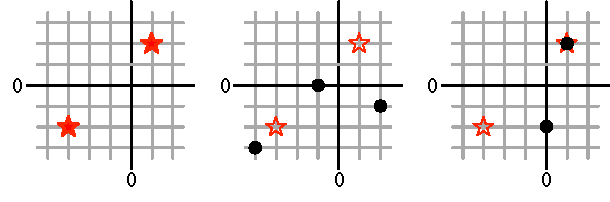
\includegraphics[width=.6\textwidth]{img/sample1.pdf}

In diesem Beispiel gibt es $k=2$ Mineralvorkommen an den Positionen $(1,2)$ und $(-3,-2)$, dargestellt als rote Sterne.
In der ersten Welle könntest du $d=3$ Sonden zu den Positionen $(-4,-3)$, $(-1, 0)$ und $(2,-1)$ schicken, die als schwarze Punkte dargestellt sind.
Diese Welle würde die folgenden $6$ Entfernungen zurückgeben: \[
  2, 4, 4, 4, 6, 10\,.
\]
In der nächsten Welle könntest du $d=2$ Sonden nach $(1,2)$ und $(0,-2)$ schicken.
Diese Welle würde die folgenden $4$ Entfernungen zurückgeben: \[
  0, 3, 5, 8\,.
\]
